\section{Puentes sobre lava caliente}

\lstset{language=C++,
	basicstyle=\ttfamily\footnotesize,
	keywordstyle=\color{blue}\ttfamily,
	stringstyle=\color{red}\ttfamily,
	commentstyle=\color{green}\ttfamily,
	numbers=left,
	breaklines=true,
	tabsize=1,
	commentstyle=\color{magenta},
	morecomment=[l][\color{magenta}]{\#}
}

\subsection{Introducci\'on}

Este problema trata sobre una competencia en la cual los participantes tienen que atravesar una serie de puentes colgantes, donde cada puente tiene una cantidad de tablones y se sabe cuáles son los tablones que están rotos en cada puente. \\
Para cruzar cada puente los participantes solo pueden saltar de tablón a tablón, y no se puede saltar a tablones que están rotos pues se caería debajo donde hay un rio de lava. También cada participante cuenta con un límite en la cantidad de tablones que puede saltar de una sola vez. \\
Los ganadores de la competencia son aquellos que crucen los puentes con la menor cantidad de saltos posibles. \\
A continuación se muestra un ejemplo con su correspondiente solución: \\

\begin{figure}[H]
  \centering
		\begin{subfigure}[b]{0.3\textwidth}
                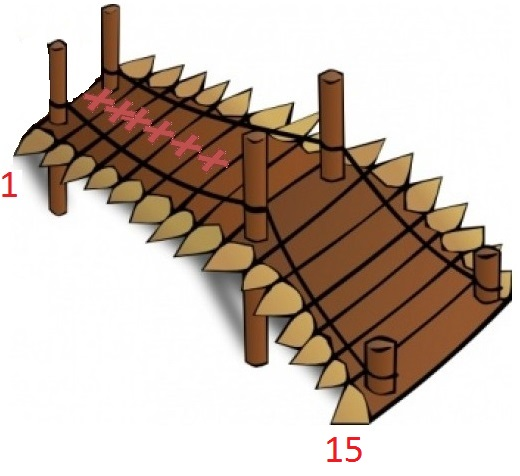
\includegraphics[scale=0.4]{Imagenes/Ej1/puenteIntro2}
                \caption{}
                \label{fig:intro}
        \end{subfigure} 
  		\begin{subfigure}[b]{0.3\textwidth}
               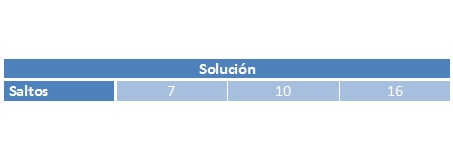
\includegraphics[scale=0.8]{Imagenes/Ej1/puenteSolu}
                \caption{}
                \label{fig:intro}
        \end{subfigure}
        \caption{Instancia de un puente con 15 tablones donde los primeros 6 estan rotos con un limite en la cantidad de tablones que se puede saltar de una vez de 7 con una posible solución} 
\end{figure}


\subsection{Desarrollo}

Este problema lo resolvimos usando una técnica golosa, la cual consiste en “saltar lo más lejos posible”, es decir que siempre que se esté en un tablón $i$ del puente con i entre 0 y n se mira si puede saltar $c$ tablones, donde c es el salto más largo que puede hacer un participante. Si el tablon número $i + c$ está sano, se procede a saltar a dicho tablón. En caso contrario se mira el tablon $i + c - 1$, es decir uno anterior y se efectúa la misma pregunta. Así sucesivamente hasta:

\begin{itemize}
	\item Saltar a un tablón sano.
	\item No poder saltar a ningún tablón, lo que implica que hay un tramo del puente donde hay $k$ tablones rotos seguidos, con $k$  $\epsilon$ $N$ y $k$ $>$ $c$. Entonces no se puede cruzar el puente
\end{itemize}

\begin{codebox}
\Procname{\textbf{Pseudoc\'odigo:}}
\li Mientras no termine de cruzar el puente
\li \ \ \ \ Si puedo saltar a algun tablon
\li \ \ \ \ \ \ \ Salto lo mas lejos posible
\li \ \ \ \ Sino
\li \ \ \ \ \ \ \ Retorno que no se puede cruzar el puente
\li Fin mientras 
\end{codebox}




\subsection{Demostraci\'on de correctitud} 

Notemos que para este problema siempre hay una solución posible, ya sea cruzar el puente o no, para toda solución donde se puede cruzar el puente requiere una cantidad de saltos determinada entonces existe al menos una solución óptima, para la solución en la que no se puede cruzar el puente esta es la solución óptima. \\
Definimos  una solución como el vector de los saltos que se realizaron para cruzar el puente ordenados por cómo se cruzaría el puente, entonces una sub solución es ser prefijo de un vector solución. Además una solución donde el vector==vacío implica que no se puede cruzar el puente. \\ \\

Nuestro algoritmo comienza con $S$=Vacío que es una sub solución de alguna solución óptima. \\
También la cantidad de tablones del puente es finita por lo que eventualmente nuestro algoritmo terminara y nos dará una solución. Esto se debe a que el algoritmo ira saltando tablones y en algún momento:

\begin{itemize}
	\item	(a) Terminara de cruzar el puente
	\item	(b) No podrá cruzar el puente
\end{itemize}

Veamos que la solución dada por el algoritmo es óptima:

(a) Dado $S$=\{ s$_{0}$,s$_{1}$,…,s$_{n}$\} alguna solución optima y $S’$=\{ s’$_{0}$,s’$_{1}$,…,s’$_{n}$\} la solución de nuestro algoritmo,

\begin{itemize}
	\item	Si $S$=$S’$ entonces nuestra solución es optima
	
	\item	Si $S$ != $S’$ entonces tomamos el primer salto donde son distintos, es decir, el primer s$_{i}$ != s’$_{i}$ con 0$\leq$ i $\leq$ n y podemos saber a qué tablón estamos saltando haciendo la sumatoria $\sum_{k=1}^{i} s_{k}$, llamemos t$_{s}$ y t$_{s’}$ a los respectivos tablones, luego como la estrategia de nuestro algoritmo es saltar lo más lejos posible $\rightarrow$ t$_{s}$ $<$ t$_{s’}$ pues si hasta el salto s$_{i-1}$, $S$-s$_{i}$ era igual a $S’$-s’$_{i}$ no puede ser que el salto s$_{i}$ llegue a un tablón más lejano porque quiere decir que s’$_{i}$ no es el salto más lejano y hubiera saltado a ese tablon. Por lo tanto en el primer salto donde difieren las soluciones, nuestro algoritmo llega a un tablón más lejano.
	
	Sabiendo esto si seguimos mirando el resto de los saltos de $S$ y $S’$ uno a uno en ningún momento puede pasar que algún s$_{j}$ llegue a un tablón t$_{p}$ posterior que s$_{j’}$ con i$<$ j $\leq$ n por la misma razón que mencionamos (como está definido nuestro algoritmo hubiera saltado a t$_{p}$), esto quiere decir que en cada salto nuestro algoritmo cae en el mismo tablón que el de la solucion optima o en alguno más adelante. \\
Finalmente llegaríamos a que con s$_{n}$ y s$_{n’}$ terminamos de cruzar el puente y como comparamos salto a salto todos los saltos de ambas soluciones, $S$ y $S’$ tienen la misma cantidad de saltos (si $S’$ tuviera menos saltos entonces $S$ no sería optima, que es absurdo porque $S$ es óptima) entonces $S’$ es solución óptima.
\end{itemize}

(b) Se debe a que hay una cantidad de tablones rotos consecutivos $>$ $c$.
Llamemos p$_{r}$ al primero de los tablones rotos consecutivos, el algoritmo ira avanzando hasta llegar al tablón anterior a p$_{r}$ e intentara saltar pero debido a que los tablones rotos consecutivos son más que lo máximo que se puede saltar no tendrá forma de hacerlo. Luego devolverá como solución que no se puede cruzar el puente, la cual es solución óptima.
 


%Para demostrar la correctitud del algoritmo veamos que \\
%Antes de empezar tengo una sub solución $S$ de alguna solución de mi problema, donde una sub solución es ser prefijo de una solución la cual es un vector con los saltos hechos. \\
%Como para este problema siempre hay alguna solución posible, ya sea cruzar el puente o no, y además para toda solución donde se cruza el puente requiere una cantidad de saltos determinada entonces existe al menos una solución óptima. En nuestro caso el algoritmo comienza con $S$=Vacío que es una sub solución de alguna solución optima. \\ \\
%Además el puente es finito y en cada iteración del algoritmo se salta alguna cantidad de tablones entonces eventualmente el algoritmo termina, que puede deberse a que (a) no pude cruzar el puente o (b) cruce el puente. \\ \\
%Por ultimo notemos que en cada momento $S$ es sub solución de alguna solución óptima \\
%Sabemos que al comenzar la k-esima iteración del algoritmo tenemos $S$ una sub solución de una solución óptima y que en esa iteración puede suceder lo siguiente:
%\begin{itemize}
%	\item no puedo saltar a ningún tablón en cuyo caso ya encontramos la solución óptima que es “no se puede cruzar el puente”
%	\item “salto lo más lejos posible” (explicado en sección 1.2) esto quiere decir que estoy agregando un salto $x$ para llegar a un tablón $j$ con $j$ entre 1 y $n$, lo que produce $S’$=$S$ $\cup$ $x$ donde $S’$ es sub solución de alguna solución óptima porque saltar lo más lejos posible genera la menor cantidad de saltos posibles para llegar a cierto tablón.
%\end{itemize}






\subsection{Complejidad}

Vamos a analizar la complejidad en peor caso de nuestro algoritmo, para esto vamos a definir los casos donde ocurre esto, que son los siguientes: \\
Sean \\
 $c$ = máxima cantidad de tablones q se puede saltar de una sola vez \\
 $n$ = cantidad de tablones del puente
\begin{itemize}
	\item \textbf{Caso 1}: Que todos los tablones del puente estén sanos y $c$ = 1
	\item \textbf{Caso 2}: Que haya una cantidad de tablones rotos consecutivos mayor a $c$ con $c < n$.
	\item \textbf{Caso 3}: Si numeramos los tablones desde 1 a $n$, que solo los tablones (1, 1+c, 1+c+1, 1+c+1+c, …) estén sanos y el resto rotos.
\end{itemize}

A continuación el extracto más importante del código para analizar la complejidad: 


\begin{codebox}
\li uint16\_t j = 0, k = 0, n = tablones.size();
\li
\li if (c $<$ n) \{
\li \ \ \ while (j $<$ n) \{
\li \ \ \ \ \ \ for(k = c; k $>$ 0; k--) \{
\li \ \ \ \ \ \ \ \ \ if ((j+k-1 $<$ n) $\wedge$ (tablones[j+k-1] != false)) \{
\li \ \ \ \ \ \ \ \ \ \ \ \ \ saltos.push\_back(j+k);
\li \ \ \ \ \ \ \ \ \ \ \ \ \ break;
\li \ \ \ \ \ \ \ \ \ \ \}
\li \ \ \ \ \ \ \ \ \}
\li \ \ \ \ \ \ \ if (k == 0) \{
\li \ \ \ \ \ \ \ \ \ \ saltos.clear();
\li \ \ \ \ \ \ \ \ \ \ break;
\li \ \ \ \ \ \ \ \ \}
\li \ \ \ \ \ \ \ j += k;
\li \ \ \ \ \}
\li \ \} else \{
\li \ \ \ \ saltos.push\_back(n);
\li \ \}
\end{codebox}


Línea 1: Son asignaciones que cuestan O(1) (la función $size$ sobre vectores de c++ tiene costo constante\footnote{http://es.cppreference.com/w/cpp/container/vector/size}) \\
Línea 3: La guarda del if son comparaciones que cuestan O(1) y el cuerpo si se cumple la guarda del if cuesta O(n) (línea 4 en cualquier caso) y sino se cumple cuesta O(1) (linea 18) $\Rightarrow$ O(1*n)=O(n) \\
Línea 6: La guarda del if son comparaciones que cuestan O(1) y el cuerpo cuesta O(1)+O(1)=O(1) (líneas 7 y 8) $\Rightarrow$ O(1*1)=O(1) \\
Línea 7: La función $push\_back$ sobre vectores de c++ tiene costo constante\footnote{http://es.cppreference.com/w/cpp/container/vector/push\_back} $\Rightarrow$ O(1) \\
Línea 12: La función $clear$ sobre vectores de c++ tiene costo lineal sobre el tamaño del vector\footnote{http://es.cppreference.com/w/cpp/container/vector/clear} $\Rightarrow$ O(n) \\
Línea 15: Es una asignación que cuesta O(1) \\
Línea 18: La función $push\_back$ sobre vectores de c++ tiene costo constante\footnote{http://es.cppreference.com/w/cpp/container/vector/push\_back} $\Rightarrow$ O(1) \\




Las siguientes líneas las analizamos dependiendo el escenario de peor caso en que estamos:

\begin{itemize}
	\item \textbf{Caso 1}:
		\begin{itemize}
			\item Línea 11: La guarda es una comparación que cuesta O(1) y como $k$=1 (por linea 5) no se cumple la guarda $\Rightarrow$ O(1)
	
			\item Línea 5: Como $c$=1 $\Rightarrow$ $k$=1 y el for solo itera 1 vez que cuesta O(1) y el cuerpo cuesta O(1) (línea 6) $\Rightarrow$ O(1). Ademas como se cumple la guarda del if de la linea 6 pues todos los tablones estan sanos, el break de la linea 8 va a cortar el for dejando $k$=1.
	
	
			\item Línea 4: $k$=1 (por línea 5) y como $j$ incrementa dependiendo de $k$ (línea 15) entonces el ciclo itera $n$ veces O(n), y el cuerpo cuesta O(1)+O(1)+O(1)=O(1) (líneas 5, 11 y 15) $\Rightarrow$ O(n*1)=O(n)
		\end{itemize}
	
	
	
	
	\item \textbf{Caso 2}: 
		\begin{itemize}
			\item Línea 11: La guarda es una comparación que cuesta O(1) y el cuerpo (por línea 5) sabemos que itera $n$ veces $\Rightarrow$ $k$=0, se cumple la guarda y el cuerpo cuesta O(n)+O(1)=O(n) (líneas 12 y 13) $\Rightarrow$ O(1*n)=O(n)
			
			\item Línea 5: Es un for que sabemos que nunca se va a cumplir la guarda de la línea 6 y entonces va a iterar $c$ veces, como el cuerpo cuesta O(1) (línea 6) $\Rightarrow$ O(c*1)=O(c) ademas sabemos que $c<n$ luego podemos acotar por $n$ $\Rightarrow$ O(n)
			
			\item Línea 4: Por línea 11 sabemos que va a cortar el ciclo con el $break$ entonces solo va a iterar 1 vez O(1), y el cuerpo cuesta O(n)+O(n)+O(1)=O(2n)=O(n) (líneas 5, 11 y 15)  $\Rightarrow$ O(1*n)=O(n)
		\end{itemize}

	
	\item \textbf{Caso 3}: 
		\begin{itemize}	
			\item Línea 11: La guarda es una comparación que cuesta O(1) y como $k>$0 (por linea 5) no se cumple la guarda $\Rightarrow$ O(1)
			
			\item Línea 5: El for va a iterar $c$ veces porque hay tramos del puente con $c$-1 tablones rotos, el cuerpo cuesta O(1) (linea 6) $\Rightarrow$ O(c*1)=O(c) \\
Tambien como siempre hay un tablon sano al que va a saltar, eventualmente en alguna iteracion se va a cumplir la guarda del if de la linea 6 terminando el for, mirando con mas detalles se ve que siempre termina con  $k$=1 o $k$=$c$.
			
			\item Línea 4: El ciclo va a iterar dependiendo de $k$ (por linea 15) que sabemos que $k$=1 o $k$=$c$ (por linea 5) entonces va a iterar $\frac{n}{c}$ veces, y el cuerpo cuesta O(1)+O(c)+O(1)=O(c) (lineas 5, 11, 15) $\Rightarrow$ O($\frac{n}{c}$*c)=O(n).
		\end{itemize}
\end{itemize}







Por lo tanto como la complejidad del algoritmo es el de la línea 3 que es \textbf{O(n)}.


%~ \subsection{Algoritmo}
%~ 
%~ \begin{lstlisting}
%~ 
%~ int main() {
	%~ string input, output;
	%~ while (getline(cin, input)) {
		%~ istringstream istr(input);
		%~ uint16_t n, c;
%~ 
		%~ istr >> n >> c;
%~ 
		%~ vector<bool> tablones(n+1);
		%~ for (uint16_t i = 0; i < n; ++i) {
			%~ uint16_t estado;
			%~ istr >> estado;
			%~ tablones[i] = (bool)estado;
		%~ }
%~ 
		%~ tablones[n] = true;
		%~ vector<uint16_t> saltos;
%~ 
		%~ puentes(tablones, c, saltos);
%~ 
		%~ if (saltos.size() > 0) {
			%~ cout << saltos.size() << " ";
			%~ for (auto& it: saltos) {
				%~ cout << it << " ";
			%~ }
			%~ cout << endl;
		%~ }
		%~ else
			%~ cout << "no" << endl;
	%~ }
	%~ return 0;
%~ }
%~ 
%~ 
%~ 
%~ 
%~ void puentes(const std::vector<bool>& tablones, uint16_t c, std::vector<uint16_t>& saltos) {
	%~ uint16_t j = 0, k = 0, n = tablones.size();
	%~ 
    %~ // caso que puedo saltar todo de una
    %~ if (c < n){
		%~ // no puedo saltar todo de una
		%~ while (j < n){
			%~ for(k = c; k > 0; k--){
				%~ if ((j+k-1 < n) && (tablones[j+k-1] != false)){
					%~ saltos.push_back(j+k);
					%~ break;
				%~ }
			%~ }
	        %~ if (k == 0){ // "No hay solucion";
	        	%~ saltos.clear();
	            %~ break;
	        %~ }
%~ 
			%~ j += k;
		%~ }
    %~ }
    %~ else {
    	%~ saltos.push_back(n);
    %~ }
%~ }
%~ \end{lstlisting}




\subsection{Testing}

Testeamos los siguientes casos de interés:
\begin{itemize}
	\item Todos los tablones sanos y $c$ = 1
	\item $c$ $>$ $n$
	\item Instancia generada aleatoriamente
	\item Instancia donde haya una parte del puente que tenga $j$ tablones continuos rotos y $c$ $<$ $j$ con $j$ $\epsilon$ $N$ 
\end{itemize}


Los test se pueden ver en el archivo: "TP1/ej1/src/tester.cpp"


\subsection{Experimentación}
Una vez hecho el análisis de la complejidad teórica, realizamos experimentos con el fin de contrastar los resultados empíricos y comprobar que el algoritmo implementado efectivamente tenía una complejidad temporal de $O(n)$. Para esto tomamos instancias aleatorias del problema, es decir se tomó una distribución discreta uniforme entre 1 y 100 y se utilizaba este valor para la cantidad de saltos del jugador. Para reducir los posibles errores de medición y evitar que los resultados se vean alterados por entradas de peor o mejor caso sesgando los resultados, se decidió tomar una cantidad fija de 5000 instancias generadas de la forma antes descrita para cada $n$ y luego tomar como estimador el promedio. En el siguiente gráfico se pueden observar los resultados del experimento:
    \begin{center}
		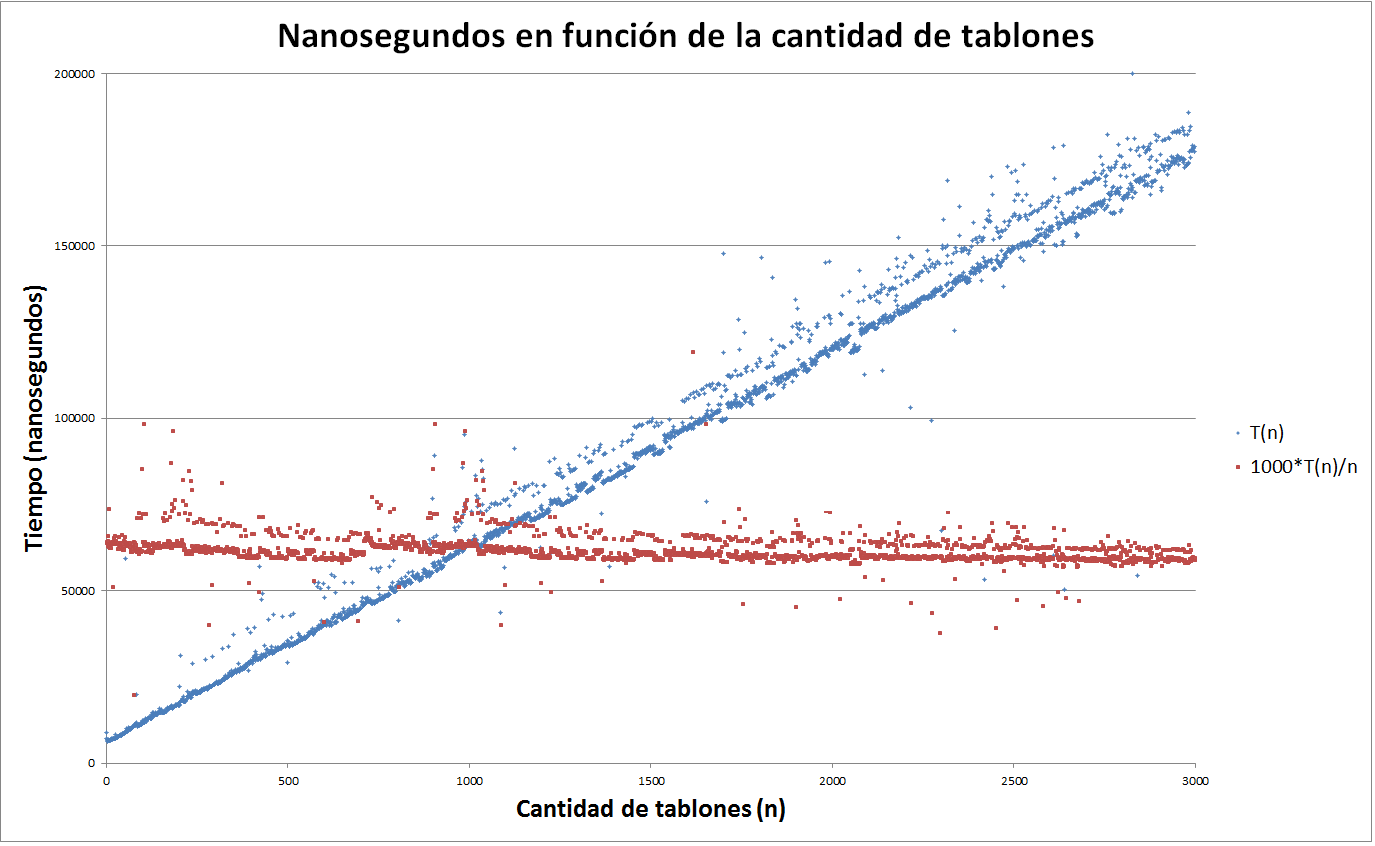
\includegraphics[scale=0.50]{Imagenes/Ej1/exp1}
		\\

		\footnotesize\textit{Gráfico de tiempos para entradas aleatorias. Notar que al graficar T(n)/n se la multiplica por 1000 para que el gráfico pueda ser apreciado con fácilidad}
	\end{center}
